\chapter{Cross-Linguistic Analysis: Translating and Training the AI Model for Multilingual Depression Detection}
\label{chap:ch3}
\par \quad In the ever-evolving field of Artificial Intelligence (AI) and Natural Language Processing (NLP), the ability to accurately detect signs of depression across different languages is both a challenge and a necessity. Multilingual depression detection hinges on the capability of AI models to understand and analyze text beyond the confines of a single language. This section delves into the critical process of translating English text into Romanian, a step essential for training our AI model to recognize depressive patterns in a multilingual context. 

We will discuss the selection criteria and the impact of utilizing a specific Translation API to bridge the language gap, thus enabling our model to process and interpret Romanian text with the same level of proficiency as English. By incorporating these translation mechanisms, we aim to enhance the model's sensitivity and accuracy in identifying depression indicators across diverse linguistic landscapes.

\section{Comparative Analysis of Translation APIs and Selection Rationale for Yandex}

\quad In our effort to refine our multilingual depression detection model, we referenced a detailed study that assessed the efficiency, accuracy, and security of various Translation APIs \cite{rashmi2020comparison}. This comparative analysis served as the foundation for selecting the most suitable API for our application, which required the translation of text from English to Romanian among other language pairs. The study meticulously compared several leading Translation APIs, including Google API, Microsoft, Systran.io, MyMemory, and Yandex, focusing on their performance in terms of speed, accuracy, security, and the breadth of language support.
\begin{itemize}
\item \textbf{Google API} emerged as a popular choice, renowned for its extensive language support, translating between over 100 languages. However, it falls short in grammar consideration and translation speed. Moreover, its security measures are deemed inadequate for handling sensitive content \cite{rashmi2020comparison}.

\item \textbf{Microsoft's Translation API} is lauded for its quality and security, offering translations among 60+ languages. It stands out for its emphasis on accuracy and stringent security protocols, although its language support is less extensive than Google's \cite{rashmi2020comparison}.

\item \textbf{Systran.io} boasts a high accuracy rate of 99\%, albeit with limitations in recognizing slang, nuances, and culturally relevant phrases. Its security is commendable, positioning it as a reliable choice for many applications \cite{rashmi2020comparison}.

\item \textbf{MyMemory} excels in translation speed but experiences the highest latency among the APIs evaluated. While it supports translations between 80+ languages, the absence of training data for certain language combinations limits its effectiveness. Nonetheless, its security is robust \cite{rashmi2020comparison}.

\item \textbf{Yandex API}, with support for 90+ languages, stands out for its balance of translation accuracy and lower latency compared to its counterparts. Despite its efficiency and broad language coverage, its security features are not optimal for translating confidential documents \cite{rashmi2020comparison}.
\end{itemize}

The conclusion from this study illuminated the strengths and weaknesses of each API, guiding our choice towards Yandex API for our multilingual depression detection model. Yandex was selected due to its free access, lower latency, and reliable accuracy across complex language pairs, making it an ideal tool for everyday translations where security is not the paramount concern \cite{rashmi2020comparison}. This choice aligns with our objective of enhancing accessibility and efficiency in depression detection across multiple languages without the need for extensive resources or development time.

Further bolstering our decision to incorporate Yandex into our multilingual depression detection framework is another rigorous study that provides a nuanced error analysis of Yandex's translations. Notably, Yandex's performance, depicted in the accompanying graph, indicates a relatively uniform distribution of errors across multiple categories \cite{cambedda2021study}. This suggests that while Yandex does have areas that require attention, such as Lexis, Syntax, and Article Usage, it generally maintains the core meaning of the translated text. This is critical for our model, which relies on the preservation of semantic content to accurately detect depressive indicators in text.

\begin{figure}[htbp]
	\centering
		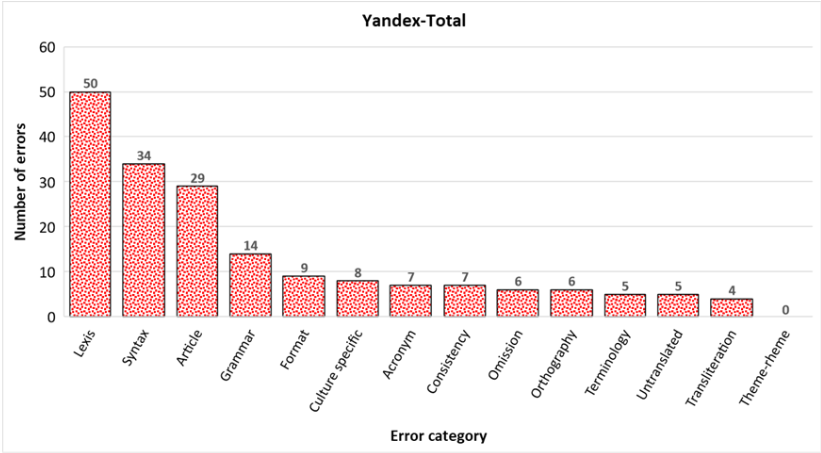
\includegraphics[scale=0.65]{LaTeX Bachelor Thesis Depression Signs Detection/figures/Yandex's-translation-performace.png}
	\caption{Yandex's translation performance \cite{cambedda2021study}}
	\label{FigGloablDepression}
\end{figure}

The Lexis category, in particular, displays the highest number of errors, signaling a need for further investigation to understand whether these issues arise from the nature of the texts or from inherent challenges within the translation tool. However, it is encouraging to note that error categories such as Grammar, Format, Culture-Specific References, Acronym, and Consistency show significantly fewer errors \cite{cambedda2021study}. These categories are essential for maintaining the integrity of meaning, which reaffirms our choice of Yandex for texts where nuanced meaning is less likely to affect the detection of depression indicators.

Further examination of the study indicates that Yandex demonstrates a more adept handling of common language texts as opposed to those with specialized jargon, registering fewer errors in translations of texts with general vernacular \cite{cambedda2021study}. Considering our dataset comprises of Reddit posts, which are typically phrased in everyday language, this finding is particularly relevant. The study also highlights that, with the exception of Article Usage, the disparity in error rates between different text types is negligible, suggesting that Yandex can reliably manage the conversational and informal style characteristic of Reddit communications.

The study’s findings underscore Yandex's capability to offer a satisfactory level of precision and effectiveness for our dataset. Given that Reddit posts are less formal, Yandex's translation services appear well-suited for our project's requirements. The platform’s proficiency in handling everyday language makes it an ideal candidate for our depression detection model's multilingual component. It provides us with a valuable tool for expanding our model’s reach, ensuring that the essence of the messages is captured, which is essential for accurate sentiment analysis, even if minute linguistic details may not be perfectly preserved.